\chapter{Reproducing the Toy Experiment}
\label{ch:reproduce_toy}

The toy experiment utilizes a standard Denoising Diffusion Probabilistic Model (\acs{DDPM} \autoref{sec:bg_diffusion}) implemented via a simple Multi Layer Perceptron (MLP) architecture.

This architecture is trained on a synthetic two-dimensional dataset consisting of a mixture of 25 distinct Gaussian modes arranged in a square grid. The training dataset comprises $100,000$ samples drawn from this underlying ground-truth distribution (\autoref{fig:toy_data}). 

\begin{figure}[!htbp]
    \centering
    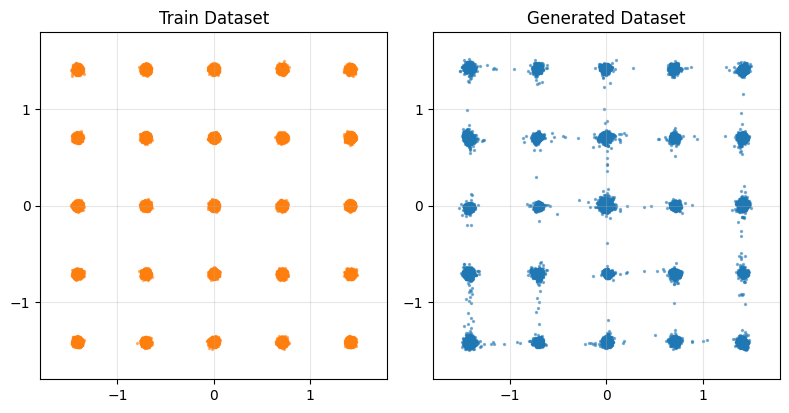
\includegraphics[width=0.6\linewidth]{figures/toy_experiment/toy_data.png}
    \caption{Train Dataset and Generated (Unfiltered) Dataset}
    \label{fig:toy_data}
\end{figure}

During the reverse diffusion process, the \acs{DDPM} occasionally interpolates between the well-defined modes, generating synthetic data points that have near-zero probability mass in the original training distribution. The primary objective of this toy setup is to investigate the effectiveness of generative uncertainty at filtering \textit{hallucinations}, defined as those \acs{OOD} mode interpolations.

\section{Code Setup}

We are trying to replicate the \emph{Toy Experiment} of \parencite{jazbec_generative_2025} which itself is based on the code provided by \parencite{aithal_understanding_2024}.

Since the code for \parencite{jazbec_generative_2025} \emph{Toy Experiment} was not available, we started from \parencite{aithal_understanding_2024} \texttt{GitHub} code and extended it to try and replicate \parencite{jazbec_generative_2025} experiment.

Unfortunately, we couldn't replicate \parencite{jazbec_generative_2025} setup fully because they did not specify every change made and parameters used. We therefore mostly went with the defaults from \parencite{aithal_understanding_2024}.

\section{Experiment Setup}

\paragraph{Creating the Ensemble}
To match what was done in \cite{jazbec_generative_2025}, We went with a Deep Ensemble \acs{DE} of $\text{M}+1=6$ models trained on the same exact reference dataset of $100{,}000$ samples.
\begin{tcolorbox}[colback=blue!10!white,colframe=blue!50!black,sharp corners]
It is important to note that a \acs{DE} behaves very differently from a \acs{LA} based ensemble in how they explore the weight space and sample models. This motivates trying the \acs{LA} on the \emph{Toy Model} later on in \autoref{ch:toy_exp_posterior}.
\end{tcolorbox}

\paragraph{Inference}
We created a dataset of pure noise and gave this pure noise dataset to all $\text{M}+1$ models to generate $2^{16}=65536$\footnote{At this stage of the thesis, it's actually $100{,}000$ generated samples but in the \autoref{ch:toy_exp_posterior} we will indeed use $65{,}536$} samples per model. We fixed the \texttt{pytorch} seed such that the inference randomness of the \acs{DDPM} is the same across the 6 models (to isolate the epistemic uncertainty properly).


\paragraph{Uncertainty Calculation}
The uncertainty was calculated as the entropy of a moment matched gaussian distribution (with diagonal approximation of the covariance) as described in \parencite{jazbec_generative_2025} method (\autoref{ch:gu_theory}). 


\section{Experiment Results}

We first show the original results from \cite{jazbec_generative_2025} to compare our results to.

\begin{figure}[!htbp]
    \centering
    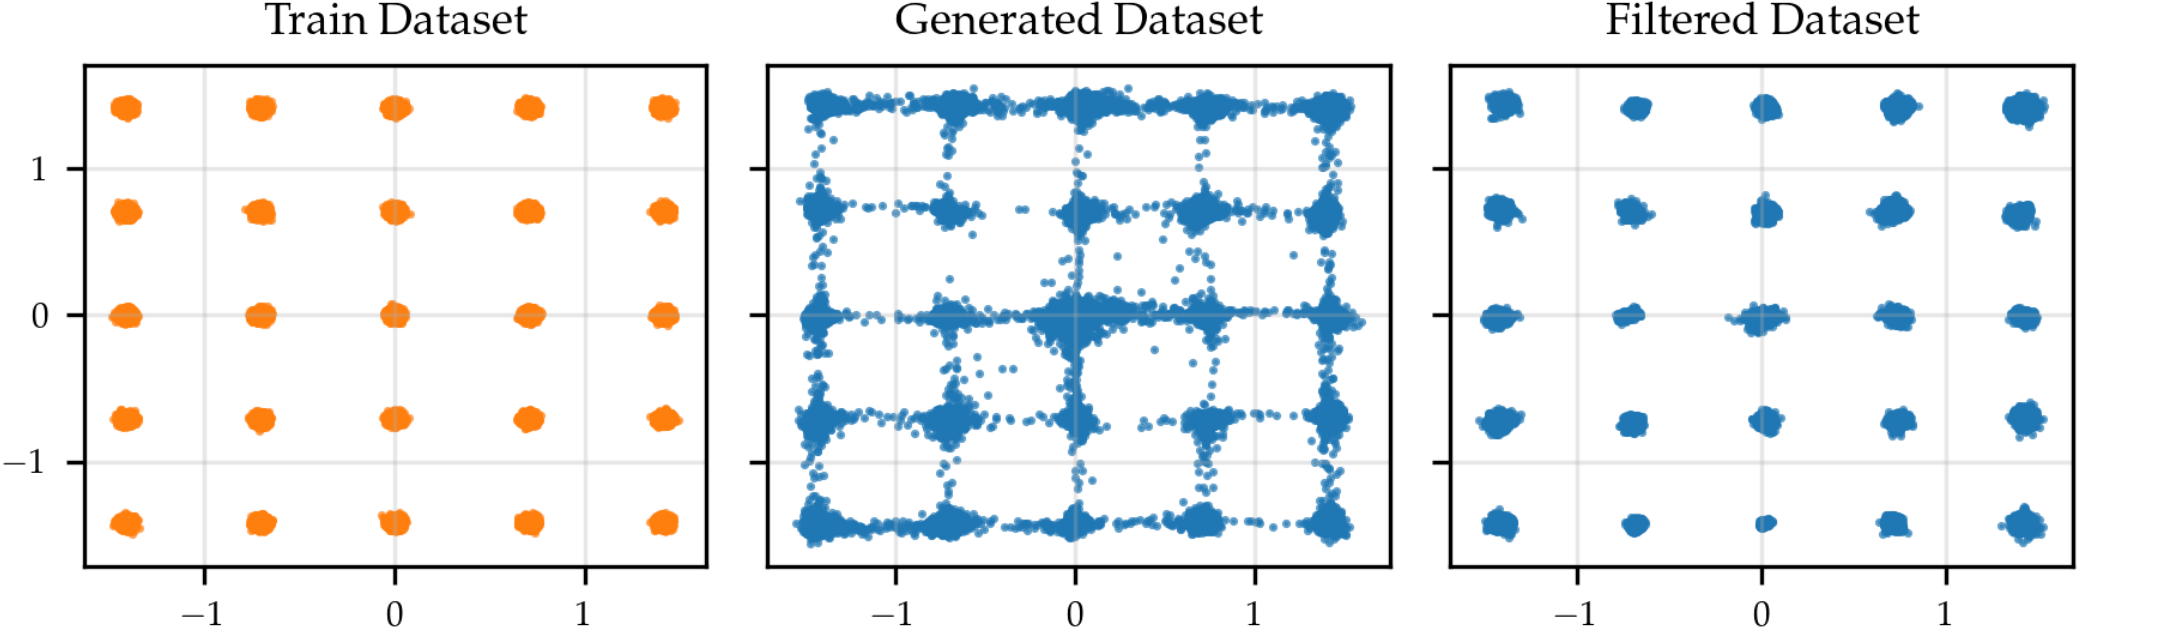
\includegraphics[width=0.9\linewidth]{figures/toy_experiment/original_jazbec.png}
    \caption{Original experiment results from \cite{jazbec_generative_2025}}
    \label{fig:toy_original_jazbec}
\end{figure}

Then we look at our results on \autoref{fig:toy_repr_de_77}. Although we couldn't replicate the high spread of \cite{jazbec_generative_2025} modes and high number of hallucinations, 
we visually are able to get similar effectiveness at filtering bad samples.  
We therefore believe our codebase is ready for further experiments.

\begin{figure}[!htbp]
    \centering
    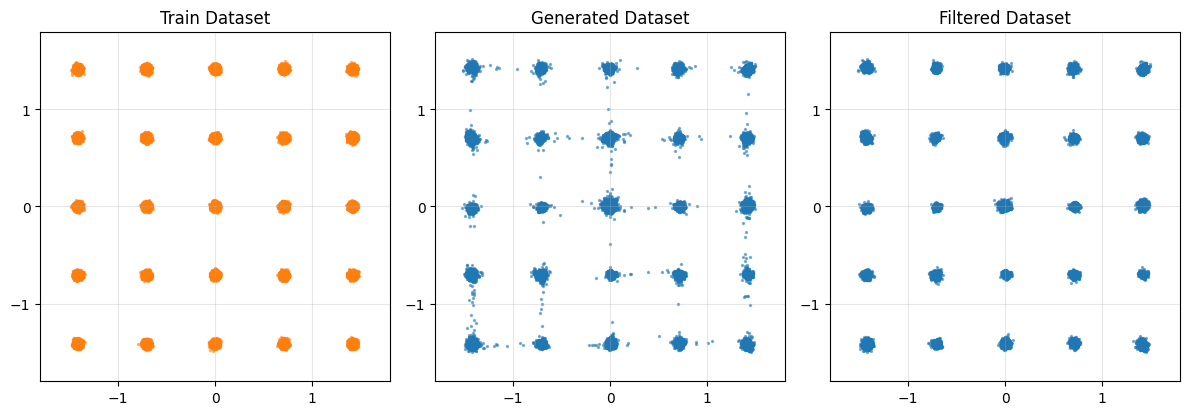
\includegraphics[width=0.9\linewidth]{figures/toy_experiment/DE_77.png}
    \caption{Result when keeping $77\%$ of the best generated samples with respect to \acs{GU} going from Generated Dataset (middle) to Filtered Dataset (right) aiming to get closer to the Training Dataset (left)}
    \label{fig:toy_repr_de_77}
\end{figure}
